\section{函数空间 \texorpdfstring{$L^{p}$}{L^p}}

参见《实变函数习题精选》徐森林

\begin{remark}
当 $1\leq p<\infty$ 时,$\lim_{ n \to \infty }f_n=f$ in $L^{p}$ 与 $\lim_{ n \to \infty }f_n (x)\underset{ m }{ = }f (x), x\in E$ 互不蕴含. 当 $p=\infty$ 时,前者蕴含后者.
\end{remark}
\begin{theorem}[$L^{p_1},L^{p_2}$ 空间包含关系]
设 $m(E)<+\infty$,且 $1\leq p_1<p_2\leq+\infty$,则 $L^{p_2}(E)\subset L^{p_1}(E)$,且
\begin{equation}
\lVert f \rVert _{p_1}\leq [m(E)]^{p_1^{-1}-p_2 ^{-1}}\lVert f \rVert _{p_2}
\label{50d515}
\end{equation}
\end{theorem}

\begin{theorem}[$L^{p}$ 空间两边夹住]
设 $f\in L^{r}(E)\cap L^{s}(E),0<\lambda<1,\frac{1}{p}=\frac{\lambda}{r}+\frac{1-\lambda}{s}$,则
\[
\lVert f \rVert _{p}\leq \lVert f \rVert _{r}^{\lambda}\cdot \lVert f \rVert _{s}^{1-\lambda}
\]
由此
\begin{equation}
\lVert f \rVert _{p}\leq \max\{ \lVert f \rVert _{r},\lVert f \rVert _{s} \}
\label{291fe9}
\end{equation}
\end{theorem}

\begin{exercise}[逐点收敛加上什么条件能推出 $L^{p}$ 收敛]
设 $1\leq p<+\infty, g\in L^{p}(E), f_n\in L^{p}(E),\lvert f_n(x) \rvert\leq g(x),n=1,2,\dots$ 在 $E$ 上, $\lim_{ n \to \infty }f_n(x)\underset{ m }{ = }f(x)$. 证明:$\lim_{ n \to \infty }f_n=f$ in $L^{p}$.
\end{exercise}
\begin{proof}
由于 $\lim_{ n \to \infty }f_n(x)\underset{ m }{ = }f(x)$. 于是逐点考虑
\[
\lim_{ n \to \infty } \lvert f_n(x)-f(x) \rvert ^{p}\underset{ m }{ = }0
\]
又因为 $\lvert f_n(x) \rvert\leq g(x)$, $n=1,2,\dots$, 故
\[
\lvert f(x) \rvert\underset{ m }{ = }\lvert \lim_{ n \to \infty } f_n(x) \rvert =\lim_{ n \to \infty } \lvert f_n(x) \rvert \leq g(x)
\]
\[
\lvert f_n(x)-f(x) \rvert ^{p}\leq [\lvert f_n(x) \rvert +\lvert f(x) \rvert ]^{p}\leq 2^{p}[g(x)]^{p}
\]
注意到 $g\in L^{p}(E), f_n\in L^{p}(E)$,由 Lebesgue 控制收敛定理可知
\[
\lim_{ n \to \infty } \int_{E}^{} \lvert f_n(x) -f(x)\rvert ^{p} \, \mathrm{d}x =\int_{E}^{} \lim_{ n \to \infty } \lvert f_n(x)-f(x) \rvert ^{p} \, \mathrm{d}x =\int_{E}^{} 0 \, \mathrm{d}x =0
\]
也就是
\[
\lim_{ n \to \infty } f_n=f\qquad \text{in }L^{p}
\]
\end{proof}

\begin{exercise}[有关 $L^{\infty}$]
设 $f \in \mathscr{L}^{\infty}(E), w(x)>0$ 且 $\int_E w(x) \mathrm{d} x=1$ .证明:
\[
\lim _{p \rightarrow+\infty}\left[\int_E|f(x)|^p w(x) \mathrm{d} x\right]^{\frac{1}{p}}=\|f\|_{\infty}
\]
\end{exercise}
\begin{proof}
因为 $f \in \mathscr{L}^{\infty}(E)$ ,故 $\|f\|_{\infty}<+\infty$ .于是
\[
\begin{aligned}
{\left[\int_E|f(x)|^p w(x) \mathrm{d} x\right]^{\frac{1}{p}} } & \leqslant\left[\int_E\left(\|f\|_{\infty}\right)^p w(x) \mathrm{d} x\right]^{\frac{1}{p}} \\
& =\|f\|_{\infty}\left[\int_E w(x) \mathrm{d} x\right]^{\frac{1}{p}}=\|f\|_{\infty} \cdot 1=\|f\|_{\infty}
\end{aligned}
\]
另一方面,对 $\forall \varepsilon>0, \exists e \subset E, m(e)>0, \mathrm{s.t}$ .
\[
|f(x)|>\|f\|_{\infty}-\frac{\varepsilon}{2}, x \in e
\]
从而可得
\[
\begin{aligned}
& \left(\int_E|f(x)|^p w(x) \mathrm{d} x\right)^{\frac{1}{p}}>\left(\int_e|f(x)|^p w(x) \mathrm{d} x\right)^{\frac{1}{p}} \\
& \geqslant\left(\|f\|_{\infty}-\frac{\varepsilon}{2}\right)\left(\int_e w(x) \mathrm{d} x\right)^{\frac{1}{p}}
\end{aligned}
\]
又因 $\lim _{p \rightarrow+\infty}\left(\int_e w(x) \mathrm{d} x\right)^{\frac{1}{p}}=1$ ,故 $\exists N \in \mathrm{~N}$ ,当 $p>N$ 时,有
\[
\left(\int_E|f(x)|^p w(x) \mathrm{d} x\right)^{\frac{1}{p}}>\|f\|_{\infty}-\varepsilon
\]
综上,当 $p>N$ 时,有
\[
\|f\|_{\infty}-\varepsilon<\left(\int_E|f(x)|^p w(x) \mathrm{d} x\right)^{\frac{1}{p}} \leqslant\|f\|_{\infty}<\|f\|_{\infty}+\varepsilon,
\]
因此
\[
\lim _{p \rightarrow+\infty}\left(\int_E|f(x)|^p w(x) \mathrm{d} x\right)^{\frac{1}{p}}=\|f\|_{\infty}
\]
\end{proof}

\begin{exercise}[$L^{p},L^{q}$ 空间的包含关系]
设 $0<p_0<q_0<\infty$,若 $L^{p_0}(E)\subset L^{q_0}(E)$ 证明对于 $0<p<q$ 有
\[
L^{p}(E)\subset L^{q}(E)
\]
\end{exercise}
\begin{note}
注意这里的包含关系和 \cref{50d515} 是相反的.
\end{note}
\begin{proof}
先证明 $m(E)<+\infty$. 反证而设 $m(E)=+\infty$,取 $E$ 中无交可测子集列 $\{ E_n \}$,s.t. $m(E_n)=1/n^3$. 作函数
\[
f(x)=\sum_{n=1}^{\infty} n^{p_0 ^{-1}+q_0 ^{-1}}\chi_{E_n}(x)
\]
易见
\[
\begin{aligned}
\lVert f \rVert ^{p_0}_{p_0} & =\sum_{n=1}^{\infty} n^{(p_0 ^{-1}+q_0 ^{-1})p_0}\cdot m(E_n) \\
 & =\sum_{n=1}^{\infty} n^{1+p_0/q_0}\cdot n^{-3} \\
 & =\sum_{n=1}^{\infty} \frac{1}{n^{2-p_0/q_0}}<+\infty 
\end{aligned}
\]
\[
\begin{aligned}
\lVert f \rVert ^{q_0}_{q_0} & =\sum_{n=1}^{\infty} n^{(p_0 ^{-1}+q_0 ^{-1})q_0}\cdot m(E_n) \\
 & =\sum_{n=1}^{\infty} n^{1+q_0/p_0 }\cdot n^{-3} \\
 & =\sum_{n=1}^{\infty} \frac{1}{n^{2-q_0/p_0}} =+\infty
\end{aligned}
\]
因此 $f\in L^{p_0}(E),f\centernot{\in}L^{q_0}(E)$. 这与 $L^{p_0}(E)\subset L^{q_0}(E)$ 矛盾.

由于这个包含关系是反的,就会有一些神奇的性质,对于 $f\in L^{p}(E)$,
\[
f^{p/p_0}\in L^{p_0}(E)\subset L^{q_0}(E)\Rightarrow f\in L^{p\cdot\frac{q_0}{p_0}}(E)\Rightarrow f\in L^{p\cdot\left( \frac{q_0}{p_0} \right)^{n}}(E),\forall n
\]
于是可以取 $n$ 使得 $p\cdot\left( \frac{p_0}{q_0} \right)^{n}>q$,再用 \cref{291fe9}  得到 $f\in L^{q}(E)$. 因此 $L^{p}(E)\subset L^{q}(E)$.

\begin{note}
事实上,利用 \cref{50d515} 可知这里 $L^{p}(E)=L^{q}(E)$.
\end{note}
\end{proof}

\begin{exercise}[利用 Holder 不等式]
设 $0<m(E)<\infty$,令
\[
N_{p}(f)=\left[ \frac{1}{m(E)} \int_{E}^{} \lvert f(x) \rvert ^{p} \, \mathrm{d}x  \right]^{1/p }
\]
证明:当 $p_1<p_2$ 时,有 $N_{p_1}(f)\leq N_{p_2}(f)$.
\end{exercise}
\begin{proof}
对于 $p_1<p_2$,记 $p=\frac{p_2}{p_1},p'=\frac{p_2}{p_2-p_1}$,则 $\frac{1}{p}+\frac{1}{p'}=\frac{p_1}{p_2}+\frac{p_2-p_1}{p_2}=1$,且
\[
\begin{aligned}
N_{p_1}(f) & =\left[  \int_{E}^{} \lvert f(x) \rvert ^{p_1}\cdot\frac{1}{m(E)}  \, \mathrm{d}x  \right]^{1/p_1} =\lVert \lvert f \rvert ^{p_1}\cdot [m(E)]^{^{-1}} \rVert_{L_1(E)}^{1/p_1} \\
 & \leq [\lVert \lvert f \rvert ^{p_1} \rVert _{L_{p}(E)}\cdot \lVert [m(E)]^{-1} \rVert _{L_{p'}(E)}]^{1/p_1}  \\
 & =\left[ \left( \int_{E}^{ } \lvert f(x) \rvert ^{p_2} \, \mathrm{d}x   \right)^{p_1/p_2 }\cdot \left( \int_{E}^{} [m(E)]^{-p'} \, \mathrm{d}x  \right)^{1/p'} \right]^{1/p_1} \\
 & =\left[ \left( \int_{E}^{ } \lvert f(x) \rvert ^{p_2} \, \mathrm{d}x   \right)^{p_1/p_2 }\cdot[m(E)]^{\overbrace{ 1/p'-1 }^{ -p_1/p_2 }}  \right]^{1/p_1} \\
 & =\left[ \frac{1}{m(E)} \int_{E}^{} \lvert f(x) \rvert ^{p_2} \, \mathrm{d}x  \right]^{1/p_2}=N_{p_2}(f)
\end{aligned}
\]
\end{proof}

\subsection{\texorpdfstring{$L^{2}$}{L^2} 空间(Hilbert 空间)}

$f, g\in L^2 (E)\Rightarrow \lvert fg \rvert\leq\frac{1}{2}(f^2+g^2)\Rightarrow fg\in L^{1}(E)$. 于是可以定义内积
\[
\left< \cdot \right>:L^2(E)\times L^2(E)\to \mathbb{R}\qquad (f,g)\mapsto\left< f,g \right>\coloneqq \int_{E}^{} f(x)g(x) \, \mathrm{d}x
\]
定义 $f,g$ 的夹角 (进而有垂直的概念)
\[
\cos\theta=\frac{\left< f,g \right> }{\lVert f \rVert _{2}\cdot \lVert g \rVert _{2}}\in[-1,1]
\]
\begin{theorem}[$L^2(E)$ 收敛蕴含弱收敛]
若 $\lVert f_n-f \rVert_{L^2(E)}\to0$ 则 $\left< f_n,g \right>\to\left< f,g \right>,\forall g\in L^2(E)$.
\end{theorem}
\begin{remark}
弱收敛不蕴含 $L^2(E)$ 收敛,也不蕴含几乎处处收敛,也不蕴含依测度收敛.
\end{remark}
设 $\{ \varphi _i:i\in \mathbb{N} \}$ 是 $L^2(E)$ 中的规范正交系\footnote{可以证明该集合至多可数}\footnote{正交意味着任意两个元垂直,规范意味着模为 1.} 对于 $f\in L^2(E)$ 定义 $f$ 关于 $\{ \varphi _i \}$ 的\textbf{广义 Fourier 系数}为
\[
c_i= \left< f,\varphi _i \right> \coloneqq \int_{E}^{} f(x)\varphi _i(x) \, \mathrm{d}x \qquad i=1,2,\dots
\]
广义 Fourier 级数为
\[
\sum_{i=1}^{\infty} c_i\varphi _i(x)
\]
\begin{figure}[H]
\centering
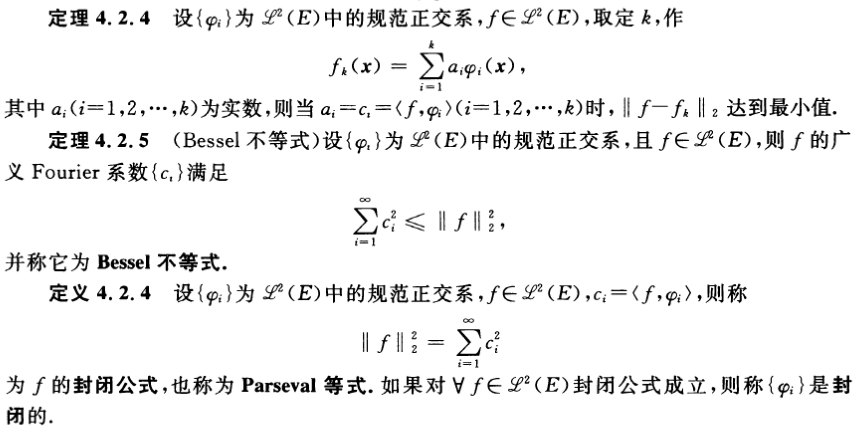
\includegraphics[width=\textwidth]{函数空间-2025040523.png}
% \caption{}
\label{}
\end{figure}

\begin{figure}[H]
\centering
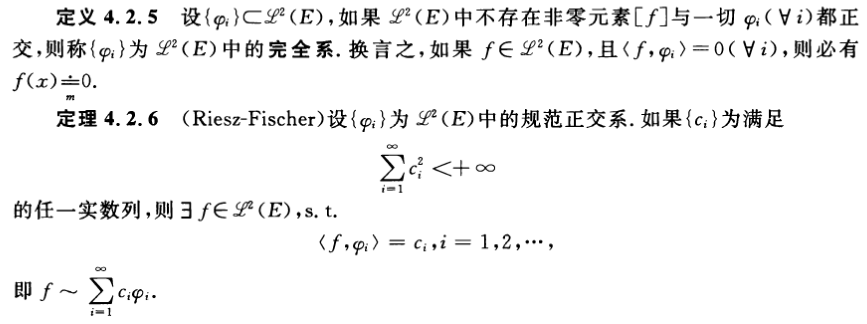
\includegraphics[width=\textwidth]{1-函数空间-2025040523.png}
% \caption{}
\label{}
\end{figure}

\begin{figure}[H]
\centering
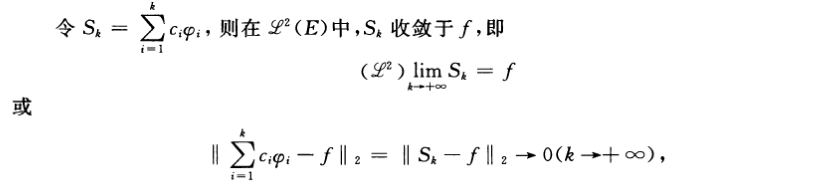
\includegraphics[width=\textwidth]{2-函数空间-2025040523.png}
% \caption{}
\label{}
\end{figure}

\begin{figure}[H]
\centering
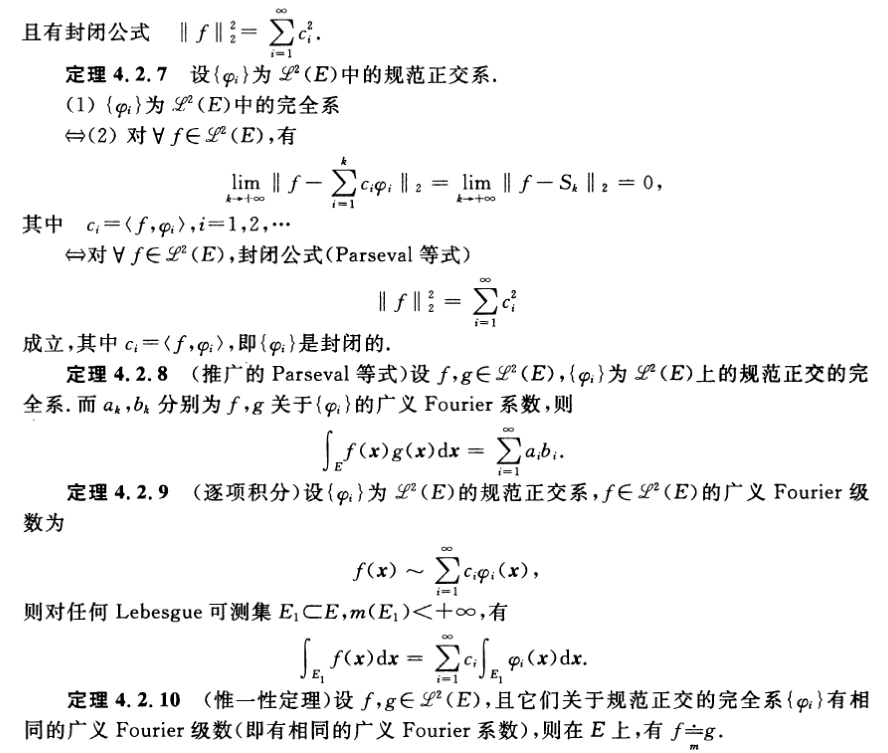
\includegraphics[width=\textwidth]{3-函数空间-2025040523.png}
% \caption{}
\label{}
\end{figure}

此处省略习题....(太多了😭)
